% A simple LaTeX template for lab reports in TDT4258 Energy Efficient Computer Design
% by Yaman Umuroglu (yamanu@idi.ntnu.no)
% Feel free to customize the style as you see fit, but the chapters/sections mentioned in the
% template should be included with the appropriate content.

\documentclass[abstract=on]{scrreprt}
\usepackage[utf8]{inputenc}
\usepackage{amsmath}
\usepackage{listings}
\usepackage{natbib}
\usepackage{graphicx}
\usepackage{color}
\definecolor{lightgray}{rgb}{0.9,0.9,0.9}

\lstset{
    basicstyle=\footnotesize\ttfamily, % Standardschrift
    numbers=left,               % Ort der Zeilennummern
    numberstyle=\tiny,          % Stil der Zeilennummern
    %stepnumber=2,               % Abstand zwischen den Zeilennummern
    numbersep=5pt,              % Abstand der Nummern zum Text
    tabsize=2,                  % Groesse von Tabs
    extendedchars=true,         %
    breaklines=true,            % Zeilen werden Umgebrochen
    keywordstyle=\color{red},
    frame=b,         
 %  keywordstyle=[1]\textbf,    % Stil der Keywords
 %  keywordstyle=[2]\textbf,    %
 %  keywordstyle=[3]\textbf,    %
 %  keywordstyle=[4]\textbf,   \sqrt{\sqrt{}} %
    stringstyle=\color{white}\ttfamily, % Farbe der String
    showspaces=false,           % Leerzeichen anzeigen ?
    showtabs=false,             % Tabs anzeigen ?
    xleftmargin=17pt,
    framexleftmargin=17pt,
    framexrightmargin=5pt,
    framexbottommargin=4pt,
    backgroundcolor=\color{lightgray},
    showstringspaces=false      % Leerzeichen in Strings anzeigen ?        
}

% Edit the meta.tex file to change title, group number and author names
% Fill in the report title, group number and student names here
\newcommand{\mytitle}{The Title of Your Report}
\newcommand{\mygroupnumber}{29}
\newcommand{\myauthor}{Kjetil Aune\\Anders Lima}

\title{\mytitle}
\author{\myauthor}
\date{\today}



\begin{document}
% The title page, edit if you want to customize it
\begin{titlepage}

\includegraphics[height=1.5cm]{images/ntnu_logo.pdf}\\[1cm]   
\begin{center}

 
% Upper part of the page
~\\[1.5cm]

\textsc{\Large TDT4258 Energy Efficient Computer Design\\Laboratory Report}\\[0.5cm]

% Set the title of the Document between two horizontal lines
\hrule ~\\[0.2cm]
{\huge \bfseries \mytitle}\\[0.4cm]		% print the title of the document
\hrule ~\\[1.5cm]

% Additional Information about the document
\begin{minipage}{0.4\textwidth}
    \centering
	\large
		\emph{Group \mygroupnumber:}\\~\\
		\myauthor
\end{minipage}

\vfill

% Bottom of the page
{\large \today}

\end{center}
\end{titlepage}


% Main matter - edit corresponding file under content/ to change
\begin{abstract}
An abstract is a short (100 to 500 words), high-level summary of the entire document. 
For this kind of report, you would start by introducing the concept that the report talks about and the goals of the work, followed by information about how the work was done and some summary of results.

This report is a hands-on approach towards learning energy efficient programming using primarily the C language. The work is done on the EFM32GG-DK3750 microcontroller from Silicon Labs, but it is applicable for programming other types of microcontrollers as well. This report describes how to utilize the on-board DAC in order to make music and sound effects, but still maintaining a low energy consumption. It is desirable to keeping the energy consumption low for a lot of reasons. Microcontrollers are used in lot of energy-sensitive areas, often battery powered, like implantable medical devices, remote controls and toys, so you want to increase their life time by decreasing the energy usage.

NEEDS TO BE WRITTEN WHEN WE HAVE RESULTS!!!

On RUNNING
\begin{itemize}
\item (Tried to down-scale, but dropped due to sound quality)
\item Reduced interrupt-frequency
\item EM1 (gets rid of 200 interrupts per note)
\end{itemize}

On IDLE
\begin{itemize}
\item Turned off DAC
\item Turned off Timer
\item EM2 (WFI)
\end{itemize}

Generated tones beforehand, so we didn't need to do a lot of heavy divisions for each boot.
Used shifting in stead of multiplication/division.
Decided using integers instead of floats for the tones.

TRY
Update linker script when disabling RAM-blocks
32.5.1 GPIO_Px_CTRL - Port Control Register
11.5.3 CMU_HFPERCLKDIV - High Frequency Peripheral Clock Division
Register

COULD TRY
Decrease voltage

\end{abstract}
\chapter{Introduction}
Your report should start with an introduction chapter that motivates the subject in general and describes the problem you are trying to solve.
\chapter{Background and Theory}

This chapter will provide information about hardware, software and different topics important for understanding the results. 

\section{Hardware}
The hardware used in this exercise is the EFM32GG-DK3750 development board from Silicon Labs depicted in Figure \ref{fig:devboard}. It was connected to a personal computer via USB. It also includes a TFT screen which can display real-time energy consumption. The EFM32GG uses the energy efficient 32-bit ARM Cortex-M3. It's worth mentioning that the M3 uses Harvard architecture \cite{cortexm3}, which allows it to read input at the same as it can execute instructions.

\subsection{Sound and DAC}
\label{sec:dac}
The board has an integrated DAC (digital-to-analog converter), which will be used for playing music and sound effects. A DAC takes input as digital data, a stream of binary values, and outputs analog values in the form of voltage or current.

Sound is best described mathematically as sine waves. These waves pushes the air at a given frequency. This frequency determines the pitch or tone. The human ear can hear sound with frequencies in the range from roughly 20Hz to 20kHz.

Since a DAC takes discrete values as input, you can generate an output that best resembles the sound by taking samples of the sine wave. The more samples you have per period, the higher the quality of the output.

\subsection{Timer and Clock}
\label{sec:timer}
The EFM32GG has a high frequency clock, HFRCLK, which is usually driven by the high-frequency oscillator HFRCO, but can also be driven by another high-frequency oscillator, or one of the low-frequency oscillator. The HFRCLK drives the prescalers that generate the high-frequency peripheral clock (HFPERCLK) and the high-frequency core clock (HFCORECLK). The HFRCLK can be divided down to run on a lower frequency, which then in turn will lower the HFPERCLK and HFCORECLK.

The EFM32GG also has 

20.3.1 Counter Modes START HERE NOW, AND DON'T WINE ABOUT BEING HUNG OVER.


\subsection{Gamepad}
In addition we had a gamepad with eight buttons and eight LEDs depicted in Figure \ref{fig:gamepad}. This was connected to the development board's GPIO pins. The gamepad includes a jumper, that when set to the lower two pins will exclude the LEDs form the power measurement. 

\begin{figure}
\centering
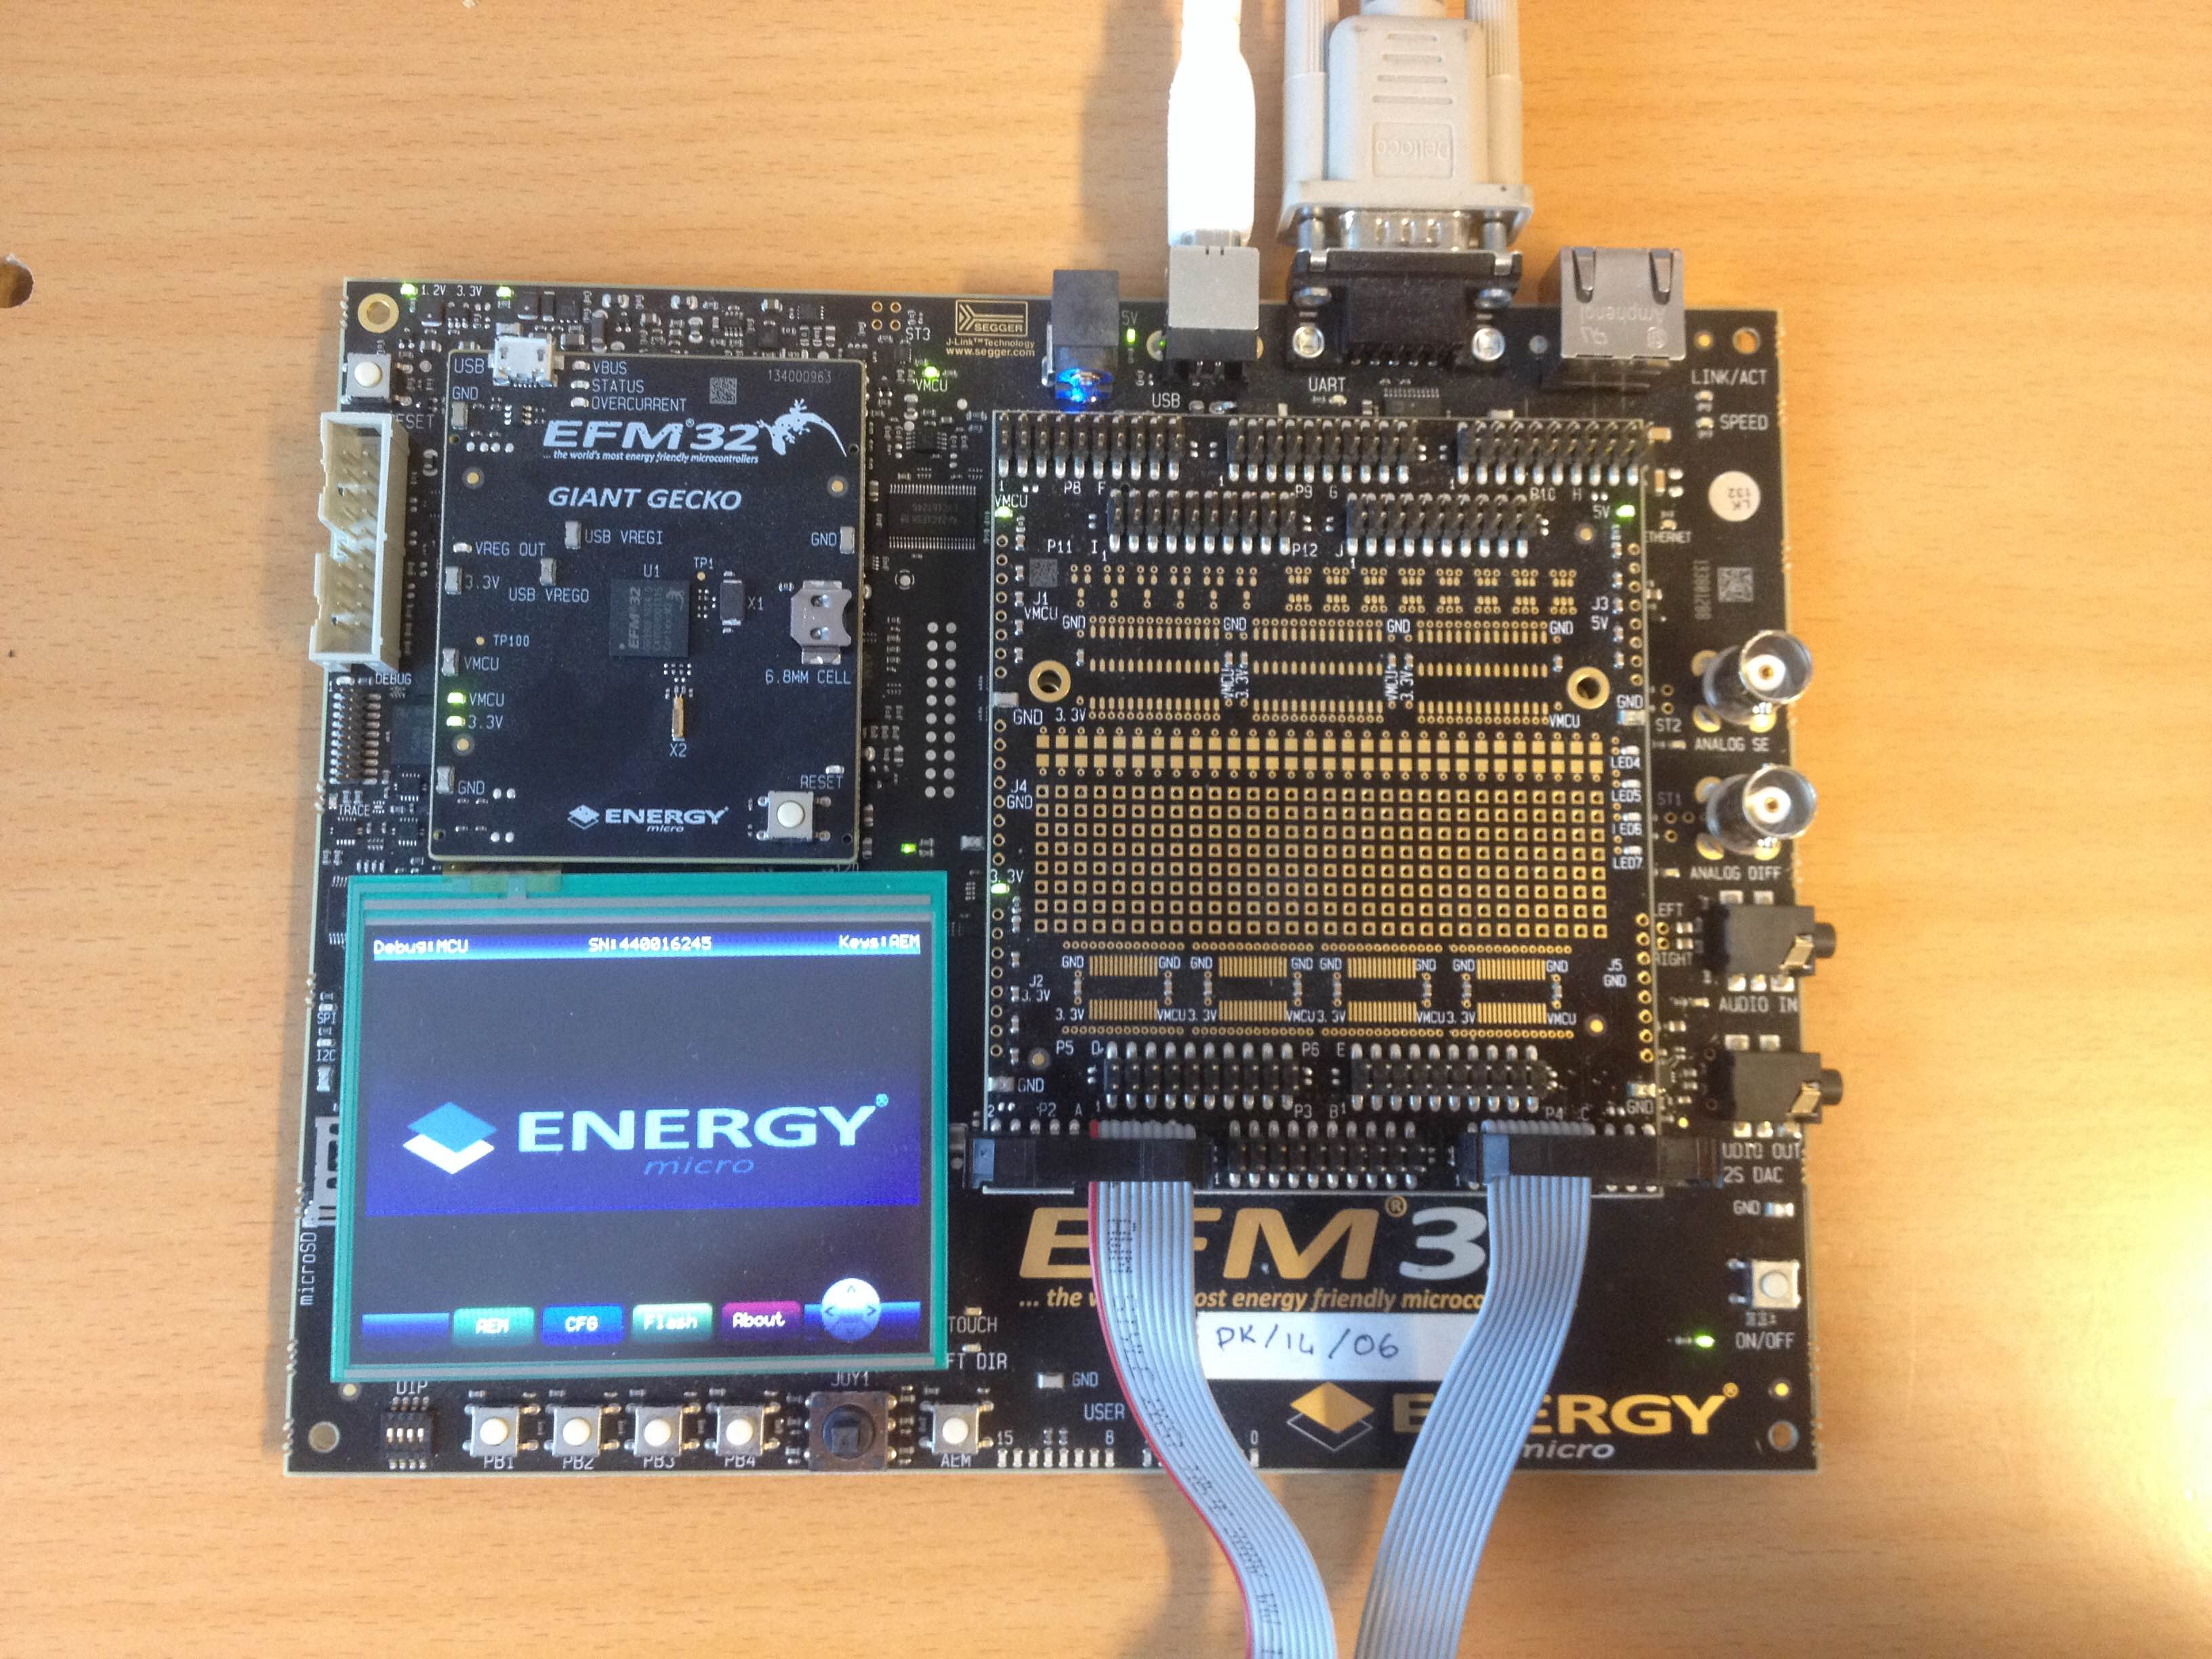
\includegraphics[scale=0.1]{images/EFM32GG-DK3750.jpg}
\caption{EFM32GG-DK3750}
\label{fig:devboard}
\end{figure}

\begin{figure}
\centering
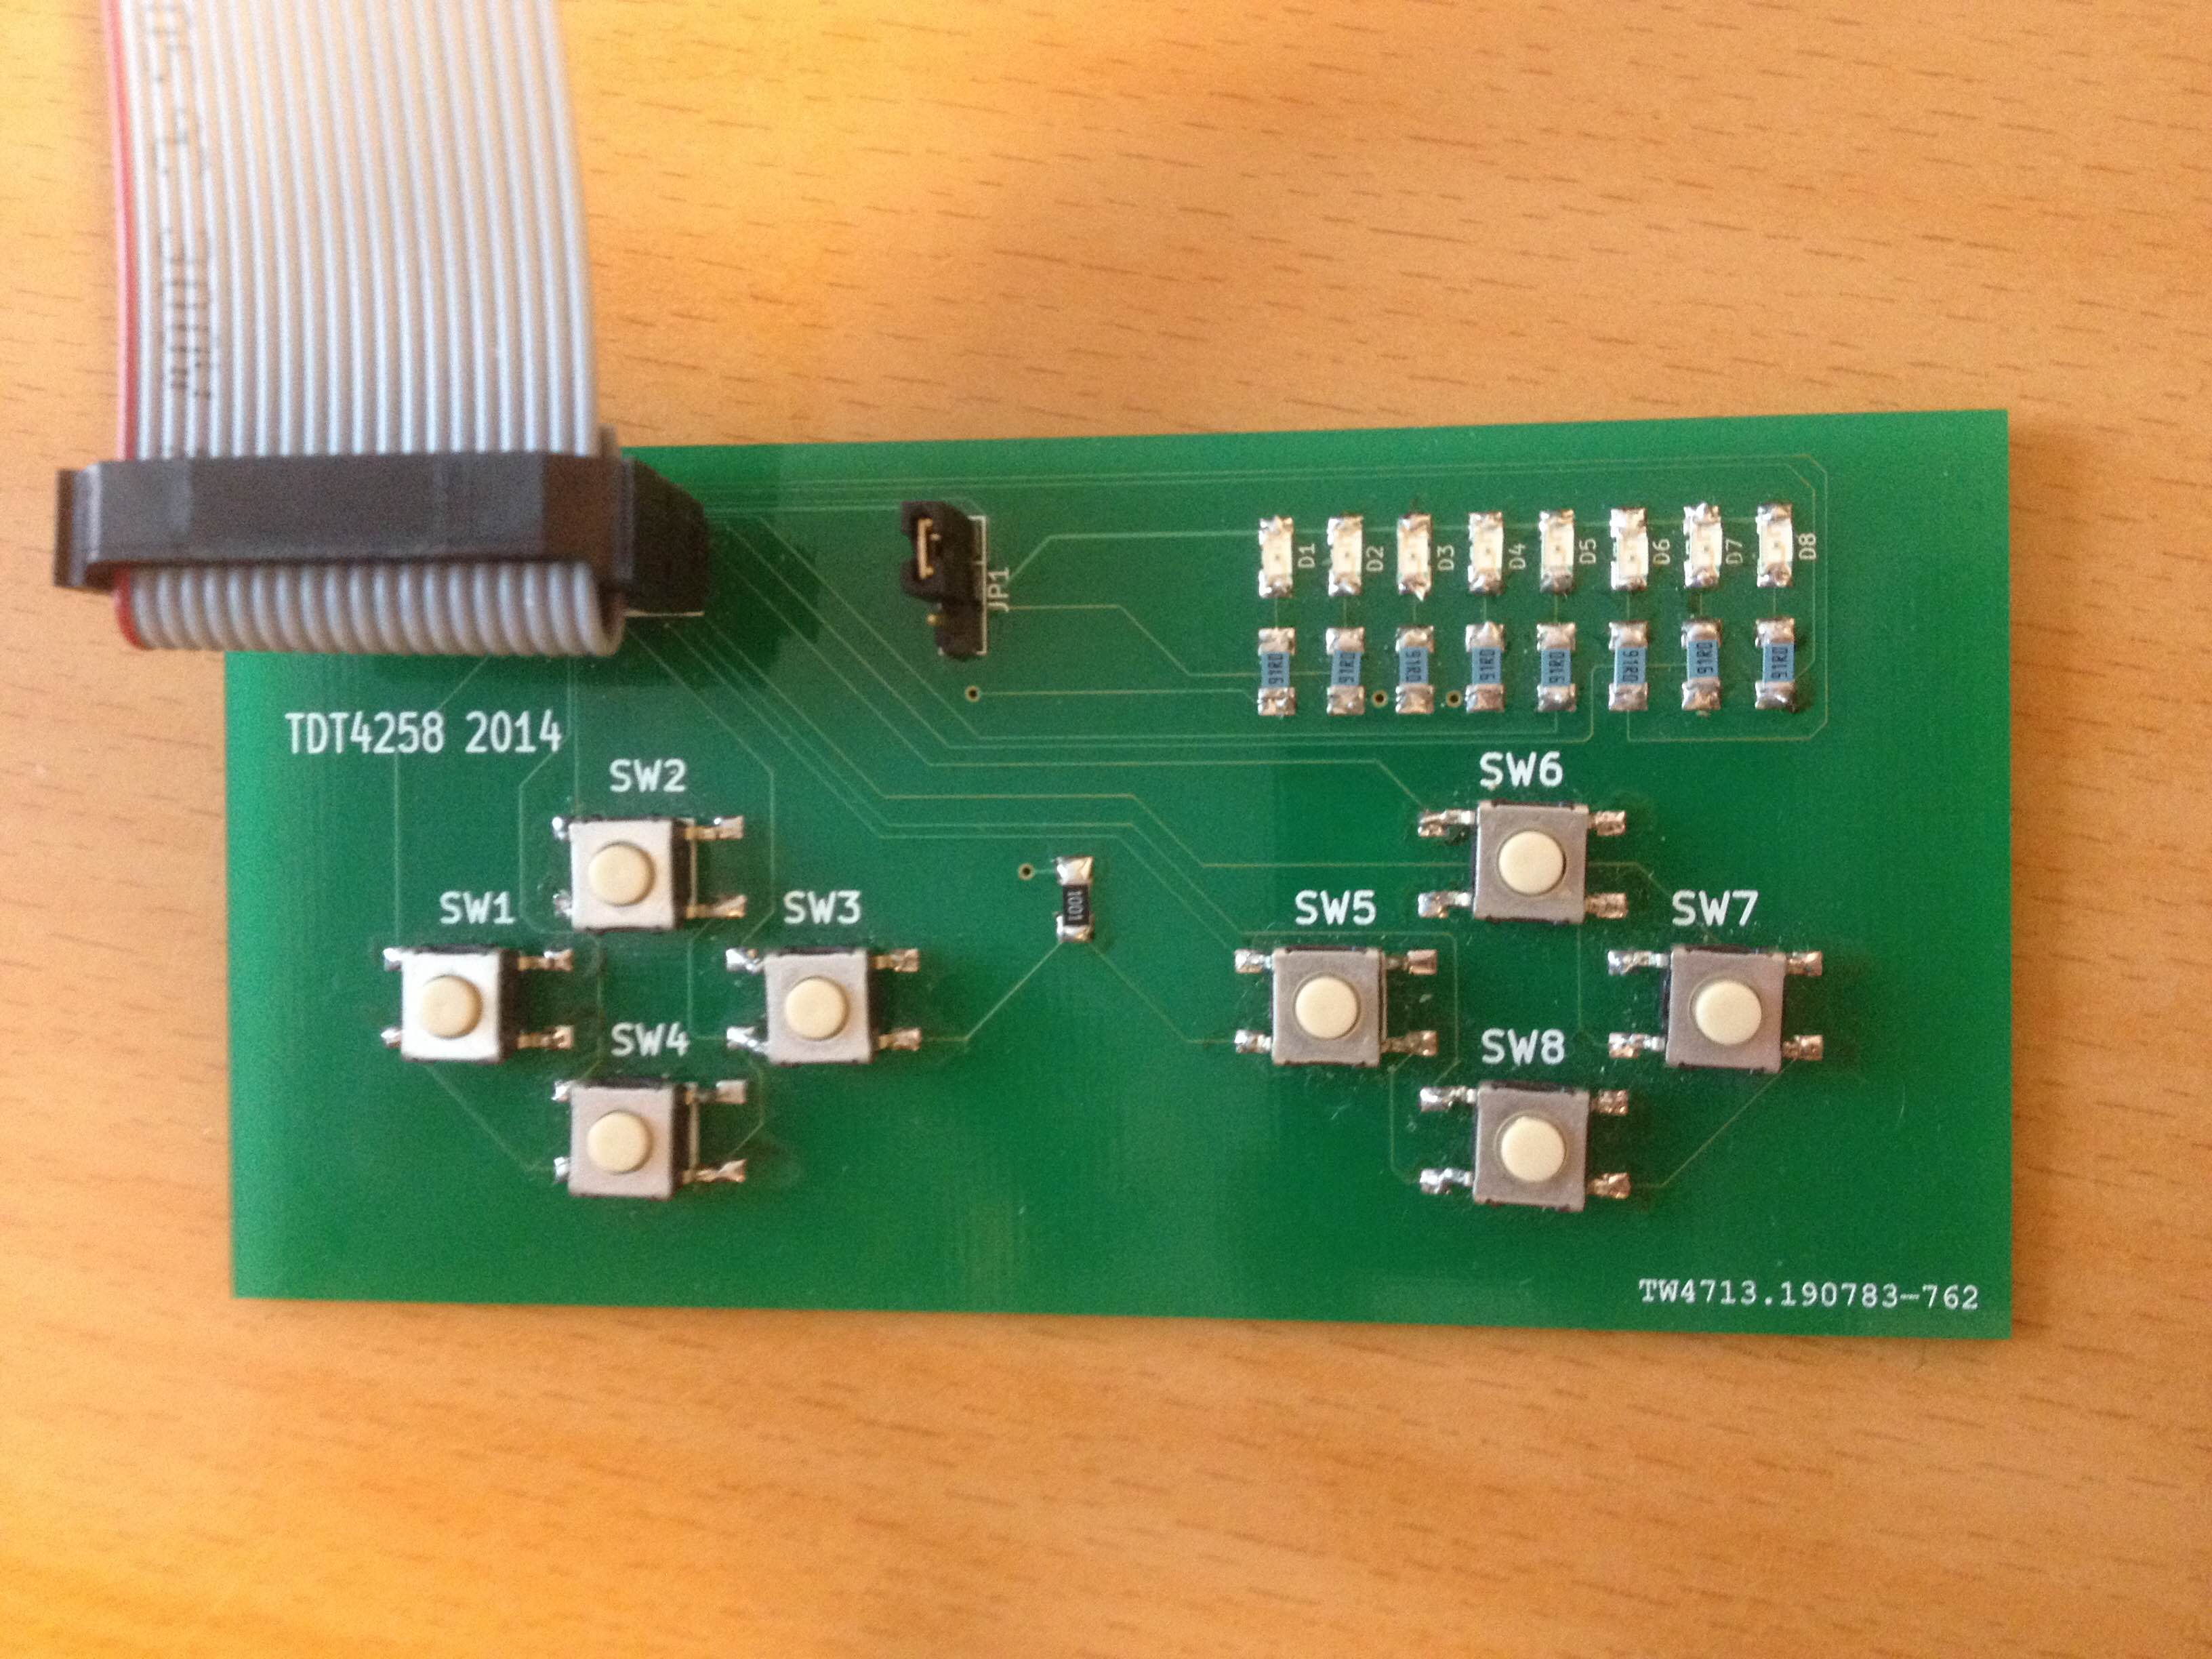
\includegraphics[scale=0.1]{images/gamepad.jpg}
\caption{Gamepad}
\label{fig:gamepad}
\end{figure}


\section{Static vs dynamic power consumption}
\label{sec:static}
The total power consumption is the sum of static- and dynamic power consumption, given by Formula 2.1, acquired from the course's lecture notes:

\begin{gather}
\label{cycle-formula}
P_{tot} = P_{dynamic} + P_{static} = \alpha C V^{2} f + I_{static} V
\end{gather}

There is static power consumption due to leakage in the transistors. The gate oxide layer in a transistor is not a perfect insulator, and therefore there will always be some current leaking through an active transistor. 

The dynamic power consumption comes from when a transistor changes state, i.e. goes from 0 to 1 or vice versa, and is dependant on the capacitance of the transistors. The thing worth mentioning is that the voltage is squared, and it is key to keep the voltage as small as possible.

The total energy consumption is given by:

\begin{gather}
\label{cycle-formula}
E = P_{total} t
\end{gather}

The static power consumption of a system is constant, but the dynamic consumption is dependant on the clock frequency. The time it takes for a certain amount of work to complete is dependent on the clock. Therefore, reducing the clock frequency will actually increase the total energy usage, because the program will need to run for a longer period. The static power consumption is present for a longer time, and as a result, it is often best to do the calculations without downscaling the clock, and then turn the components off.

\section{The C language}
C is a low-level, imperative programming language. It is a general purpose language, which also provides a lot of control for the programmer with regards to memory control and memory access. A very useful part of C is pointers. Pointers contain addresses to memory locations, and can be dereferenced to obtain the value on the given location. This is very useful when programming microcontrollers, because it makes it easy to write and obtain values directly from memory.

\section{Energy Efficiency}

There are a lot of ways of reducing the power needed to run programs, and the following section describes some of these techniques.

\subsection{Energy Modes on the EFM32GG}
The EFM32GG has five different energy modes, all with different levels of active components and power consumption. Figure \ref{fig:em} shows an overview of the EFM32GG and Figure \ref{fig:em2} shows a color scheme with the different energy modes indicated with a respective number. The colors in Figure \ref{fig:em} translates to the highest energy mode in which they are active.

Here are some of the key aspects worth noticing about each energy mode:

\begin{description}
  \item[EM0 - Run] Everything is active.
  \item[EM1 - Sleep] The CPU is sleeping, the rest is active.
  \item[EM2 - Deep Sleep] High frequency oscillators, flash memory, timer/counter are inactive
  \item[EM3 - Stop] RAM, DAC and external interrupts are still active.
  \item[EM4 - Shutoff] Everything is shut off, only a reset can turn it on again.
\end{description}

\begin{figure}[h]
\centering
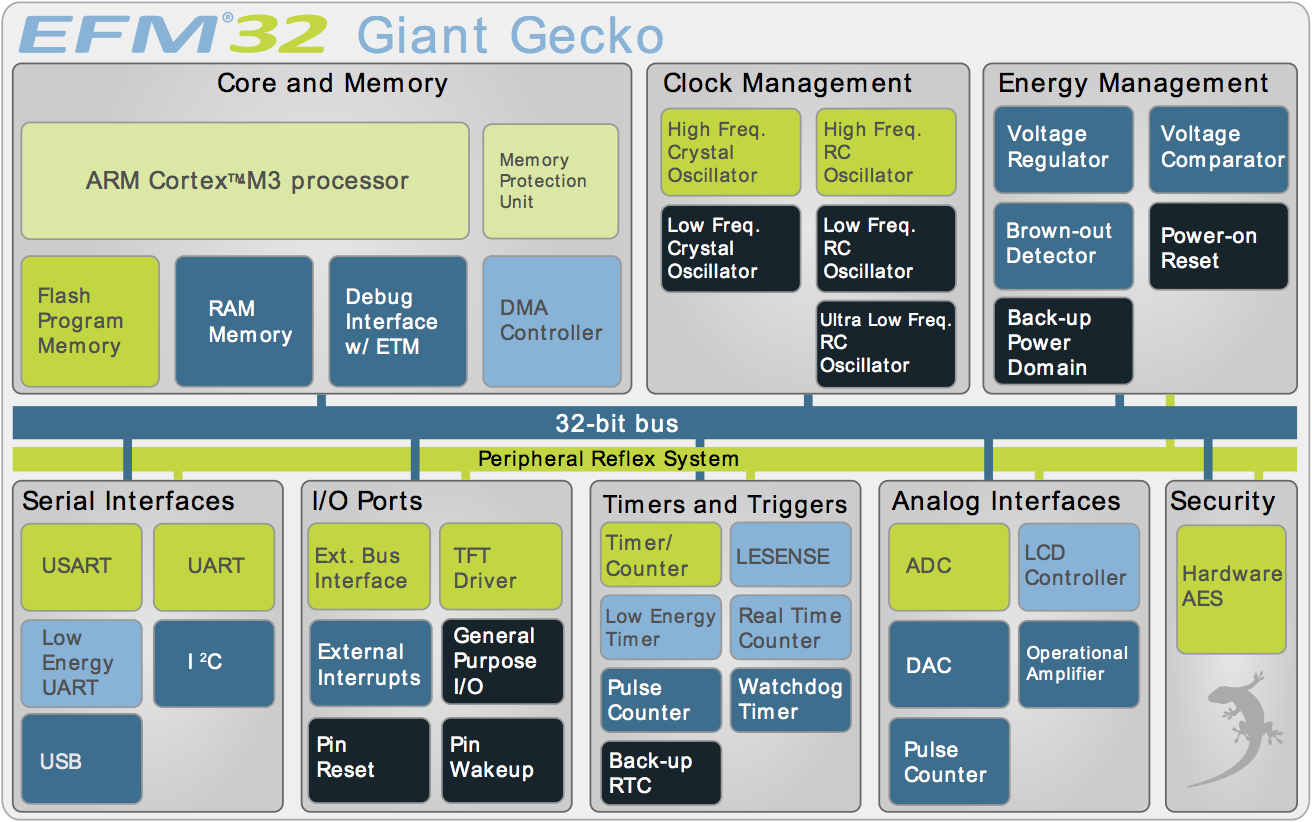
\includegraphics[scale=0.6]{images/em.png}
\caption{Diagram of EFM32GG}
\label{fig:em}
\end{figure}

\begin{figure}[h]
\centering
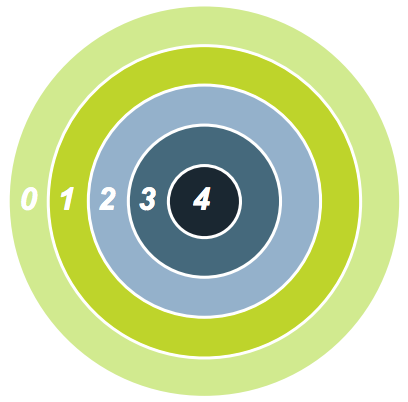
\includegraphics[scale=0.6]{images/em_numbers.png}
\caption{Energy Mode Indicator}
\label{fig:em2}
\end{figure}

\subsection{Interrupts}
\label{sec:interrupts}
When a program is idle, there are several ways to wake it up. One way is by using polling. Polling is when you repeatedly check the status of a unit to see if there are any changes or if it is ready for use. This is not very efficient with regards to energy efficiency, because you continuously check to see if there is work to be done, and you use a lot of processing power. 

A good replacement for polling is the use of interrupts. An interrupt is a signal to the processor indicating that an event needs immediate attention. When the processor receives an interrupt signal, it suspends its current program and executes a handler routine defined in the interrupt handler vector. After the handler routine is completed, the processor returns to the program it was originally executing\cite{wolf2012computers}. The use of interrupts will relieve the processor of a lot of work, and only do work when it's needed, which in turn decreases the energy consumption.

\subsection{Reducing Static Power Consumption}
As described in Section \ref{sec:static}, there is always static power consumption when a transistor is active. One way of reducing the total energy consumption, is by simply turning off parts of the system that are not in use, and thus decreasing the total static power consumption. 
\chapter{Methodology}
This chapter will describe the workflow, and a detailed explanation of our implementation. At the end of this chapter we will discuss the testing of our implementation.
\section{Workflow and project structure}
The code were mostly written in Emacs on Ubuntu 14.04 LTS running in VirtualBox on a Windows8.1 laptop. Git was used to transfer files between the virtual machine and other computers used write code.

The file structure is shown in \ref{code:structure}. 
\begin{lstlisting}[caption={Project structure}, label={code:structure}]
|-- buttons.h
|-- core
|-- dac.c
|-- efm32gg.h
|-- ex2.bin
|-- ex2.c
|-- gpio.c
|-- interrupt_handlers.c
|-- lib
|   |-- efm32gg.ld
|   |-- ex2.bin
|   |-- libefm32gg.a
|-- Makefile
|-- songs.h
|-- timer.c
|-- tone-generator.py
|-- tones.h
\end{lstlisting}

\subsubsection{Header files}
All the header files are used to store predefined variables. efm32gg.h contains memory locations for the most used registers. 
tones.h contains implementation specific values for the different tones used, explained further in section \ref{sec:generating}. 
songs.h contains a struct, defining how we store songs, and also contains the songs and sound effects used in this exercise.
buttons.h contains the register values on different key presses, for easy comparison on GPIO interrupt.

\subsubsection{C-Files}
ex2.c is the main file, which is run at power-on. 
gpio.c, timer.c and dac.c has code for setting up and powering on and off the different parts.
interrupt_handlers.c contains the code for handling interrupts, which is also the code that actually plays the sound.

\subsection{Bulding and flashing}
\label{sec:bulding}
The GNU-Toolchain was used to compile and build the C-code. This was done using the \texttt{make} command. The binary was then uploaded to the board, via USB, using Silicon Labs' eACommander.

\subsection{Debugging}
We were not able to install the gdb tool for ARM on the virtual machine. This made debugging quite hard, and lead to a try and fail approach. If we needed to know the value of a variable or a register, we wrote the binary value to the gamepad's LEDs.

\section{Implementation}
To get started, and to get familiar with programing a microcontroller using the C language, we reimplemented the functionality of Exercise 1 \cite{ex1}. This included the setup of GPIO, clocks and interrupts.

\subsection{Setting Up}
To make thing work, we need to run some initial code to set things up. 
\subsubsection{GPIO}
To make the General-Purpose-Input-Output work, we first enable the GPIO clock by setting a value to the CMU register.
Then we enable high drive strength and set pin 8 to 15 as output, on Port A, for the gamepad's LEDs. We also need to make the buttons work, which is done by writing some values to GPIO\_PA registers.
Finally we enable interrupt on button presses.

\subsubsection{DAC}
Next we set up the DAC. We need the high peripheral clock to drive this as well. 

\subsection{Generating sound}
\label{sec:generating}
Our next goal was to get a simple tone playing. As explained in section \ref{sec:dac} sound is moving air. To get the 440Hz tone we wanted, we need to change the value in the DAC 880 times per second. This makes a square pulse with a period of 440Hz.
To make this happen, we made use of the timer explained in section
\ref{sec:timer}. We sat TIMER1\_TOP to 140, which gave us 100000 interrupts per second.
In the interrupt handler we used two counters one to keep track of when to feed a new value to the DAC, and one for when to change the tone.
We used a tone generator script written in python \ref{app:py} to generate a header file with the values for each tone. These values indicates how many interrupts there should be between each time we feed a new value to the DAC.

\subsubsection{}

\subsection{Improvements}

\subsubsection{}

\section{Testing}
Add content in this section that describes how you tested and verified the correctness of your implementation, with respect to the requirements of the assignment.
\begin{figure}
\centering
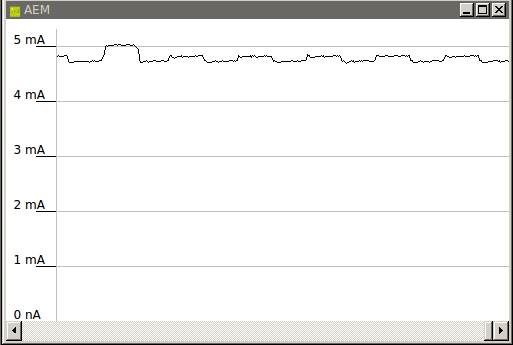
\includegraphics[scale=1]{images/Idle_preEF.PNG}
\caption{A JPEG image of a galaxy. Use vector graphics instead if you can.}
\label{fig:universe}
\end{figure}
\chapter{Results}
In this chapter, you should discuss the results you have obtained from your implementation.
These can be correctness results, i.e whether the implementation behaved as expected, or numerical results that express runtime or energy measurements.
\chapter{Conclusion}
This chapter should be a look back at the entire report and summarizing the problem, the solution and the obtained results.

\section{Evaluation of the Assignment}
You can include comments about the assignment itself here. While this part is not obligatory and not graded, it is valuable feedback to the course staff that can be used to improve the exercises in the future.


% Bibliography - edit references.bib and use the \cite command in text
\bibliographystyle{plain}
\bibliography{references}

\chapter*{A Appendices}
\section*{1 Code}
\lstinputlisting[language=Python, label={code:python}, caption={Python script for generating tones.h}]{Code/tone-generator.py}

\lstinputlisting[language=C, label={code:ex2}, caption={The main file}]{Code/ex2.c}

\lstinputlisting[language=Python, label={code:python}, caption={Python script for generating tones.h}]{Code/tone-generator.py}

\lstinputlisting[language=Python, label={code:python}, caption={Python script for generating tones.h}]{Code/tone-generator.py}

\lstinputlisting[language=Python, label={code:python}, caption={Python script for generating tones.h}]{Code/tone-generator.py}
\end{document}
